\chapter{Knot selection in compartmental spline models: osteoarthritis of the knee}
\label{applications-con_fit_splines}

Chapter~\ref{applications-splines_knot_loc} and
\ref{applications-priors_knots_select} demonstrated the importance of
knot selection in spline models for sparse, noisy data. In this
chapter, we return to this point in the context of compartmental
models where the age-specific hazards are represented by splines and
the parameter of primary interest, prevalence, comes from the solution
to a system of differential equations based on these splines. In this
setting, modeling decisions about knots in one parameter affect all
the other parameter estimates.  The consistent model for
osteoarthritis of the knee provides a demonstration of how subtle this
can be.

Osteoarthritis (OA) is joint disorder that affects joint cartilage and
underlying bone.  OA causes pain in the joints and limits movement.
Osteoarthritis of the knee is common and it causes significant
morbidity, particularly in the
elderly. \cite{felson_epidemiology_1988, felson_incidence_1995}
Systematic review yielded $602$ data points representing $27$ countries
in $10$ GBD 2010 Study regions.

Since OA knee is so rare in young adults, expert priors inform the
model that the onset of the disease starts at age 30.  The number and
location of knots in the incidence rate after this minimum age of
onset determine critical features of the model. As shown in Figure
\ref{fig:app-oa knee knots}, it is important to have enough knots to
represent the rapid change in age-specific incidence.

    \begin{figure}[h]
        \begin{center}
            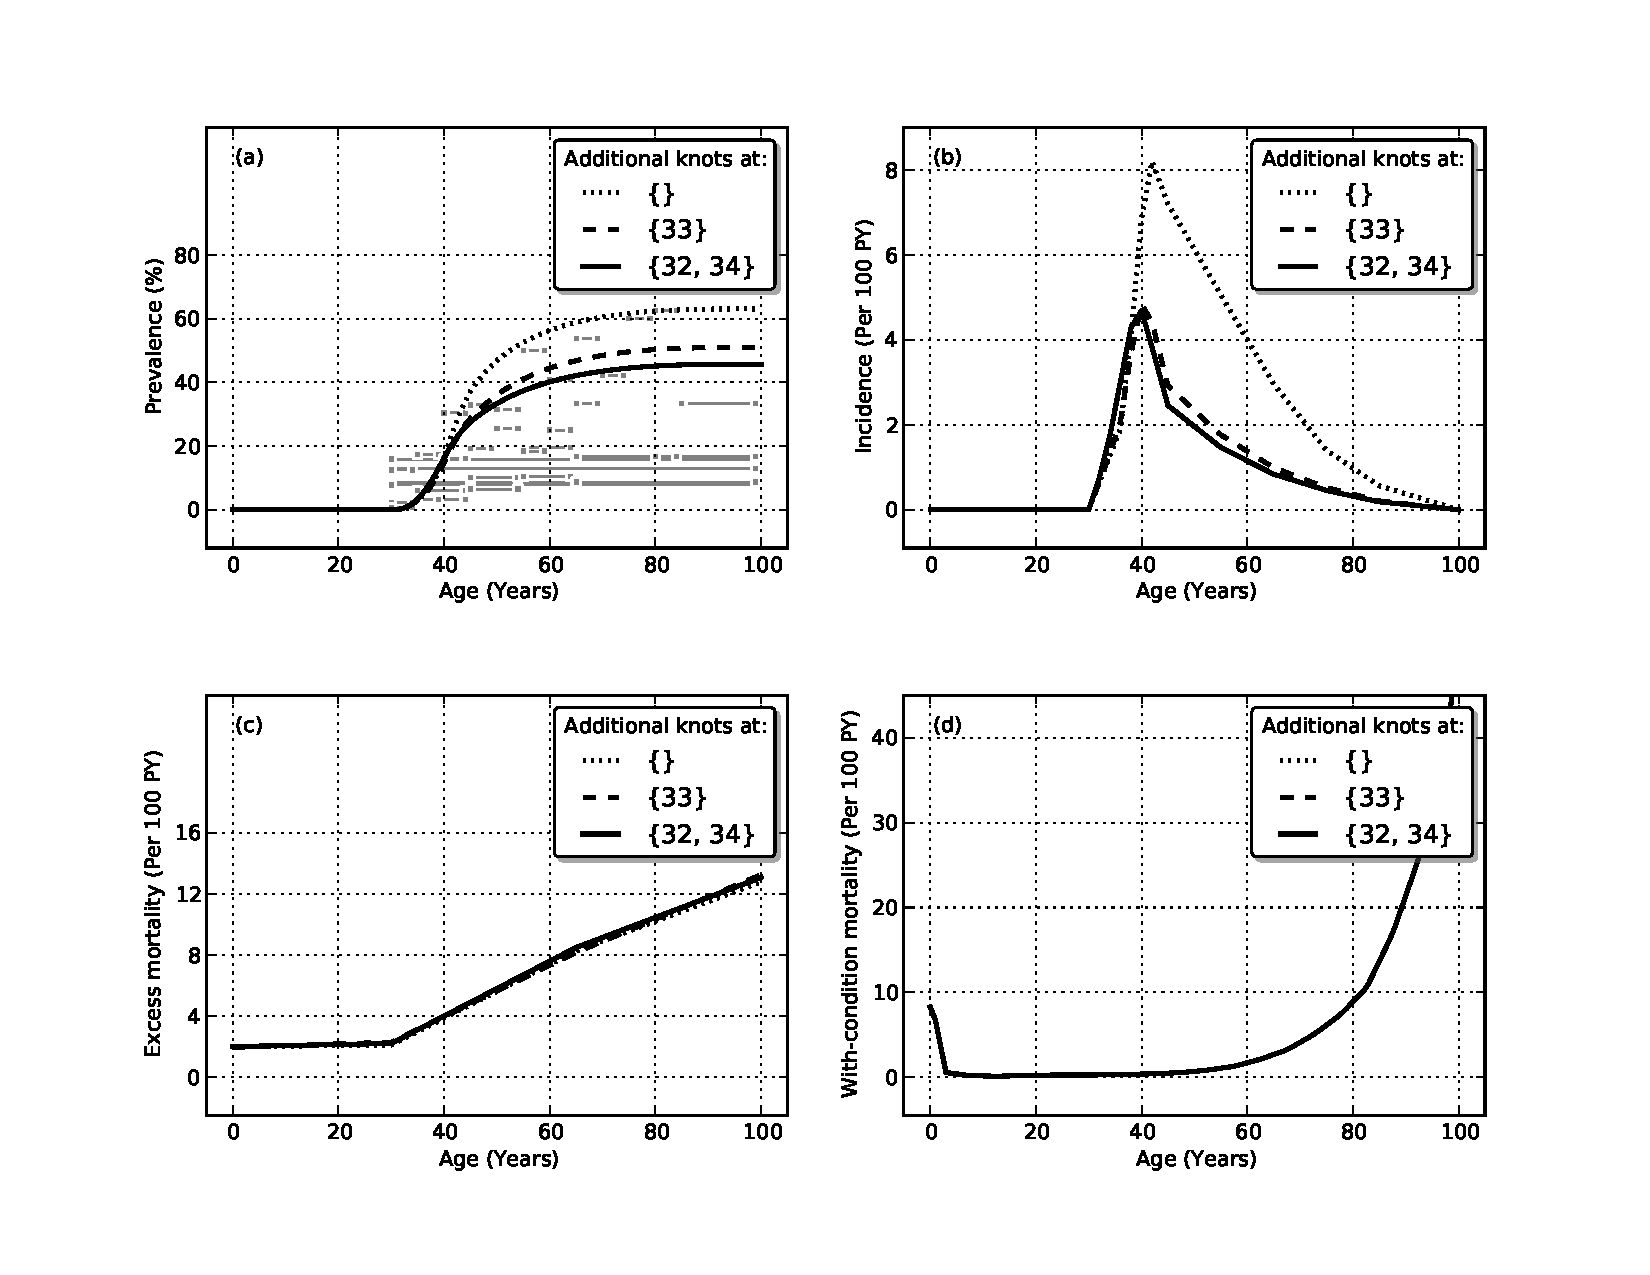
\includegraphics[width=\textwidth]{oa_knee-knots.pdf}
            \caption{Knot selection between the ages of 30 and 99
              plays an important role in the estimates of OA knee
              parameters.  Prevalence estimates appear
              in panel (a) and incidence in panel (b) for females in
              South Asia with osteoarthritis of the knee in 2005.  The
              incidence rate of all models has knots at \{0, 30, 35,
              40, 45, 65, 100\}.  Between the ages
              of 30 and 35, the models have additional knots at \{\}, \{31\}
              or \{33\}.}
            \label{fig:app-oa knee knots}
        \end{center}
    \end{figure}

The model is also sensitive to assumptions about the epidemiological
profile, expressed in the model as expert priors.  Figure
\ref{fig:app-oa knee priors} compares assumptions about OA knee
incidence.  A prior that requires zero incidence at ages greater than
99 implies that incidence decreases with age.  In other words, after a
certain age, if OA knee hasn't developed, it is unlikely it ever
will. Without this prior, incidence increases with age.  The logic
requirement of internal consistency in the compartmental model means
that prevalence estimates are also affected as shown in Figure
\ref{fig:app-oa knee priors}.

    \begin{figure}[h]
        \begin{center}
            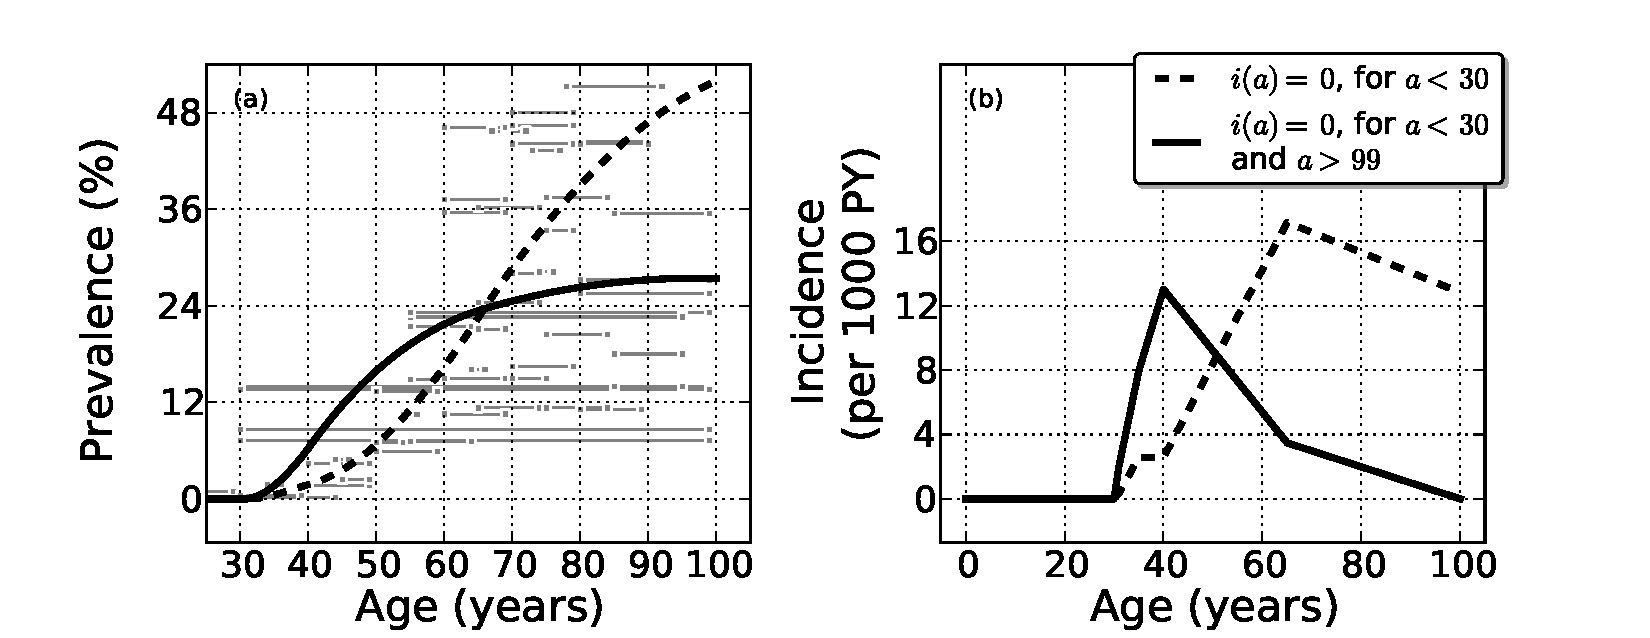
\includegraphics[width=\textwidth]{oa_knee-i_prior.pdf}
            \caption{A comparison of compartmental models with and
              without a prior stipulating no onset of the disease in
              ages greater than 99.  Prevalence (panel (a)) and
              incidence (panel (b)) estimates for South Asian females
              with OA knee in 2005.}
            \label{fig:app-oa knee priors}
        \end{center}
    \end{figure}

TK concluding remarks